% Definiciones y constantes de estilo
% Clase del documento
\documentclass[a4paper,12pt,twoside,openright,titlepage]{book}

% Paquetes necesarios
\usepackage{eurosym}
\usepackage[utf8]{inputenc}
\usepackage[spanish]{babel}
\usepackage[hidelinks,colorlinks,citecolor=Fuchsia,urlcolor=blue,linkcolor=Cerulean]{hyperref}
\usepackage{listings}
\usepackage{color}
\usepackage{anysize}
\usepackage{fancyhdr}
\usepackage{cite}
\usepackage{multirow}
\usepackage{titlesec}
\usepackage[cmex10]{amsmath}
\usepackage{algorithmic}
\usepackage{textcomp}
\usepackage{enumerate}
\usepackage{fixltx2e}
\usepackage{emptypage}
\usepackage{float}
\usepackage[pdftex]{graphicx}
\usepackage{array}
\usepackage{mdwmath}
\usepackage[caption=false,font=footnotesize]{subfig}
\usepackage{fixltx2e}
\usepackage{pdfpages}
\usepackage{quotchap}
\usepackage{fancybox}
\usepackage[acronym]{glossaries}
\usepackage{appendix}
\usepackage{bookmark}

% Euro (€)
\DeclareUnicodeCharacter{20AC}{\euro}

% Estilo de la bibliografía
\bibliographystyle{IEEEtran}

% Inclusión de gráficos
\graphicspath{{./graphics/}}

% Extensiones de gráficos
\DeclareGraphicsExtensions{.pdf,.jpeg,.jpg,.png}

% Definiciones de colores (para hidelinks)
\definecolor{LightCyan}{rgb}{0,0,0}
\definecolor{Cerulean}{rgb}{0,0,0}
\definecolor{Fuchsia}{rgb}{0,0,0}

% Keywords (español e inglés)
\def\keywordsEn{\vspace{.5em}
{\textbf{\textit{Key words ---}}\,\relax%
}}
\def\endkeywordsEn{\par}

\def\keywordsEs{\vspace{.5em}
{\textbf{\textit{Palabras clave ---}}\,\relax%
}}
\def\endkeywordsEs{\par}


% Abstract (español e inglés)
\def\abstractEs{\vspace{.5em}
{\textbf{\textit{Resumen ---}}\,\relax%
}}
\def\endabstractEs{\par}

\def\abstractEn{\vspace{.5em}
{\textbf{\textit{Abstract ---}}\,\relax%
}}
\def\endabstractEn{\par}

% Estilo páginas de capítulos
\fancypagestyle{plain}{
\fancyhf{}
\fancyfoot[CO]{\footnotesize\emph{\nombretrabajo}}
\fancyfoot[RO]{\thepage}
\renewcommand{\footrulewidth}{.6pt}
\renewcommand{\headrulewidth}{0.0pt}
}

% Estilo resto de páginas
\pagestyle{fancy}

% Estilo páginas impares
\fancyfoot[CO]{\footnotesize\emph{\nombretrabajo}}
\fancyfoot[RO]{\thepage}
\rhead[]{\leftmark}

% Estilo páginas pares
\fancyfoot[CE]{\emph{\pieparcen}}
\fancyfoot[LE]{\thepage}
\fancyfoot[RE]{\pieparizq}
\lhead[\leftmark]{}

% Guía del pie de página
\renewcommand{\footrulewidth}{.6pt}

% Nombre de los bloques de código
\renewcommand{\lstlistingname}{Código}

% Definiciones de funciones para los títulos
\newlength\salto
\setlength{\salto}{3.5ex plus 1ex minus .2ex}

\newlength\resalto
\setlength{\resalto}{2.3ex plus.2ex}

% Corrección warning
\setlength{\headheight}{15pt} 

% Estilo de sección
\newcommand{\lsection}[1]
                {\section{#1}
                \vskip-.9\resalto % Corrección del posible salto por defecto de \section
                \hrule
                \vskip+.9\salto} % Vuelvo ha realizar el salto

% Estilo de los acrónimos
\renewcommand{\acronymname}{Glosario}
\renewcommand{\glossaryname}{Glosario}
\pretolerance=2000
\tolerance=3000

% Pie de tabla
\addto\captionsspanish{
\def\tablename{Tabla}
\def\listtablename{\'Indice de tablas}
}

% Traducir appendix/appendices
\renewcommand\appendixtocname{Apéndices}
\renewcommand\appendixpagename{Apéndices}

% Definiciones de comandos
\newcommand{\nombreautor}{Juan Sidrach de Cardona Mora}
\newcommand{\nombretutor}{Dr. Sergio López-Buedo}
\newcommand{\nombretrabajo}{Interfaz web para la gestión de sondas de red de altas prestaciones}
\newcommand{\fecha}{Junio 2014}
\newcommand{\grado}{Doble Grado en Ingeniería Informática y Matemáticas}
\newcommand{\grupoInvestigacion}{High Performance Computing and Networking Research Group}
\newcommand{\departamento}{Dpto. de Tecnología Electrónica y de las Comunicaciones}
\newcommand{\facultad}{Escuela Politécnica Superior}
\newcommand{\universidad}{Universidad Autónoma de Madrid}
\newcommand{\pieparizq}{\href{https://github.com/JSidrach/NetWatcher}{\scriptsize{github.com/JSidrach/NetWatcher}}}
\newcommand{\pieparcen}{Trabajo de Fin de Grado}
\newcommand{\logoizq}{Logo_EPS}
\newcommand{\logoder}{Logo_UAM}
\newcommand{\correo}{***REMOVED***}

% Glosario y acrónimos
\makeglossaries
% Acrónimos

\newacronym{HTTP}{HTTP}{Hypertext Transfer Protocol}
\newacronym{URL}{URL}{Uniform Resource Locator}
\newacronym{FPGA}{FPGA}{Field-Programmable Gate Array}
\newacronym{IFG}{IFG}{InterFrame Gap (pausa temporal entre paquetes)}
\newacronym{RAID}{RAID}{Redundant Array of Independent Disks}
\newacronym{pcap}{pcap}{Packet capture (formato de traza, utilizado por programas como \textit{Wireshark} y \textit{tcpdump})}
\newacronym{API}{API}{Application Programming Interface (métodos públicos de una aplicación)}
\newacronym{JSON}{JSON}{JavaScript Object Notation}
\newacronym{PHP}{PHP}{PHP Hypertext Pre-processor}
\newacronym{AJAX}{AJAX}{Asynchronous JavaScript and XML}

% Glosario

\newglossaryentry{bitstream}{name={bitstream},description={En este contexto se refiere al binario que configura el Hardware de la FPGA}}
\newglossaryentry{traza}{name={traza},plural={trazas},description={Archivo que contiene paquetes de red capturados}}
\newglossaryentry{simple}{name={simple},description={Formato de traza que acepta la FPGA utilizada}}
\newglossaryentry{servicioweb}{name={Servicio Web},description={Conjunto de métodos remotos accesibles a través de la red}}
\newglossaryentry{proxy}{name={proxy},description={Servidor que sirve de intermediario entre las peticiones de recursos que realiza un cliente a otro servidor}}
\newglossaryentry{framework}{name={framework},description={Entorno software que proporciona una funcionalidad base para facilitar la organización y desarrollo de aplicaciones}}
\newglossaryentry{back-end}{name={back-end},description={Componentes internos de la aplicación que procesan los datos provenientes del front-end}}
\newglossaryentry{front-end}{name={front-end},description={Interfaz, parte de la aplicación que interacciona directamente con el usuario}}
\newglossaryentry{script}{name={script},plural={scripts},description={Programa interpretado que se almacena en un archivo de texto plano}}

% Inicio del documento
\begin{document}

% Elección del idioma (español)
\selectlanguage{spanish}

%
% Portada
%
\pagenumbering{gobble}
%
% Portada
%

% Universidad, Facultad
\begin{titlepage}
\selectlanguage{spanish}
\begin{center}
\textbf{\begin{huge}
\universidad \\
\end{huge}}
\bigskip
\begin{LARGE}
\facultad \\
\end{LARGE}
\end{center}

\bigskip
\bigskip

%
% Imágenes (logos) izquierdo y derecho
%
\begin{figure}[h]
  \begin{center}
    \includegraphics[scale=0.35]{\logoizq}
    \hspace{1cm}
    \includegraphics[scale=0.4]{\logoder}
  \end{center}
\end{figure}

\bigskip
\bigskip
\bigskip

% Grado
\begin{center}
\begin{large}
\textbf{\grado}\\
\end{large}
\end{center}

\bigskip

\textbf{\begin{center}
\begin{huge}
\MakeUppercase{Trabajo de Fin de Grado}
\end{huge}
\end{center}}

\bigskip
\bigskip

% Nombre del TFG
\begin{center}
\textbf{\begin{large}
\MakeUppercase{\nombretrabajo}\\
\end{large}}
\end{center}

% Nombre del autor
\vspace{\fill}
\begin{center}
\textbf{\nombreautor}\\
% Tutor
\textbf{Tutor: \nombretutor}\\
% Ponente, si está definido en main.tex
\ifcsname nombreponente\endcsname
\textbf{Ponente: \nombreponente}\\
\fi

\bigskip

% Fecha
\textbf{\fecha}\\
\end{center}
\end{titlepage}

% Primera página
\pagenumbering{Alph}
\thispagestyle{empty}
\par\vspace*{\fill}
\begin{flushleft}
\begin{scriptsize}
\end{scriptsize}\end{flushleft}
\newpage
\thispagestyle{empty}
\begin{center}

% Nombre del trabajo
\textbf{\begin{large}
\MakeUppercase{\nombretrabajo}\\*
\end{large}}
\vspace*{0.2cm}
\vspace{5cm}

% Nombre del autor y del tutor
\large Autor: \nombreautor \\*
\large Tutor: \nombretutor \\*
\ifcsname nombreponente\endcsname
\large Ponente: \nombreponente\\
\fi

\vfill

% Grupo de investigación, departamento, facultad, universidad y fecha
\ifcsname grupoInvestigacion\endcsname
\grupoInvestigacion \\
\fi
\departamento \\
\facultad \\
\universidad \\
\vspace{1cm}
\fecha \\

\clearpage

\end{center}
\normalsize


%
% Agradecimientos
%
\pagenumbering{Roman}
\setcounter{page}{0}
\chapter*{Agradecimientos}

TODO: Agradecimientos.

Lorem ipsum dolor sit amet, consectetur adipiscing elit. Phasellus laoreet dolor at sodales porta. Morbi facilisis hendrerit lacus vel sollicitudin. Aenean eleifend urna metus, eget vestibulum libero dictum tincidunt. Curabitur quis ultrices lorem. Duis ultricies, eros eget condimentum pharetra, tellus eros lobortis nulla, vel mattis nibh dui et felis. Interdum et malesuada fames ac ante ipsum primis in faucibus. Nam non lorem et ligula condimentum molestie. Fusce quis dolor non metus suscipit commodo. Praesent vel pulvinar lectus. Nullam ac dui eget magna accumsan volutpat. Aliquam sed purus quis lorem dictum rutrum auctor eu enim. Pellentesque a urna ac ligula cursus lacinia. Aenean sodales justo massa, vel imperdiet justo imperdiet ut. Nulla euismod pulvinar arcu eu convallis. Vivamus a tempus nunc, et vulputate nulla.

Sed dapibus aliquam imperdiet. Vivamus est quam, fermentum vitae augue id, ultricies tincidunt massa. Praesent tincidunt ex sem, ut aliquet nulla imperdiet eu. Duis ac ultricies lorem. Aenean consequat ipsum nec arcu aliquam, sit amet interdum quam tempus. In justo odio, bibendum vel nulla nec, aliquet tristique justo. In vel metus ut libero suscipit ultricies.

Class aptent taciti sociosqu ad litora torquent per conubia nostra, per inceptos himenaeos. Proin urna elit, iaculis id quam at, pretium laoreet ipsum. Phasellus ultricies faucibus ex et eleifend. Quisque facilisis erat dolor, ac rhoncus erat convallis et. Aliquam semper eleifend imperdiet. Sed eros ipsum, sagittis in pellentesque vel, vestibulum a augue. Duis sapien mauris, fringilla a tortor ut, sollicitudin volutpat nunc. Pellentesque vestibulum vel arcu in molestie. Nullam fermentum dolor luctus metus efficitur pulvinar. Pellentesque risus enim, tempus id ullamcorper in, maximus id nisl. Cras rhoncus consequat augue eu gravida. Ut efficitur mauris vitae orci dignissim sagittis. Suspendisse vitae massa eget nunc bibendum interdum.

Vestibulum quis turpis sed diam facilisis convallis. Class aptent taciti sociosqu ad litora torquent per conubia nostra, per inceptos himenaeos. Vivamus congue tellus nec lobortis feugiat. Nam hendrerit ullamcorper tempus. Proin maximus, lacus at tempor pellentesque, sem nisi facilisis lorem, sagittis tristique mauris dui at est. Class aptent taciti sociosqu ad litora torquent per conubia nostra, per inceptos himenaeos. Mauris pellentesque lobortis leo, ac dictum urna tempus id. Curabitur sed ante leo. Proin laoreet nisi nec dictum auctor. Mauris lacinia erat ut massa viverra, nec tempus metus elementum. Cras ut blandit justo, in pretium massa. In hac habitasse platea dictumst. Donec malesuada viverra quam, in ultricies libero. Phasellus finibus velit in sem tempus mattis at tristique ligula.

% Cita
\begin{flushright}
\textit{``In the beginning the Universe was created.
This has made a lot of people very angry and been widely regarded as a bad move.''}
-- Douglas Adams
\end{flushright}
  

%
% Resumen
%
% Resumen en inglés
\chapter*{Abstract}

\begin{abstractEn}
TODO: Resumen en inglés, 250-500 palabras.

Lorem ipsum dolor sit amet, consectetur adipiscing elit. Aliquam malesuada libero auctor sapien volutpat, sed fringilla enim tristique. Aliquam varius lorem in risus tempus egestas. Aenean accumsan elementum diam vel commodo. Nulla lectus sapien, finibus ac mauris non, efficitur venenatis felis. Donec at rutrum dolor, a lobortis arcu. In fermentum hendrerit bibendum. Phasellus eget arcu quam. Maecenas vulputate sapien eu dictum pulvinar. Suspendisse sit amet neque a turpis efficitur dapibus ut et turpis.

Vestibulum commodo faucibus tellus vitae consequat. Donec purus enim, hendrerit vitae feugiat sed, sagittis in tortor. Duis sed ex non ligula cursus dapibus. Etiam pellentesque suscipit dolor, vel facilisis est ornare sed. Nullam eleifend tellus non elementum efficitur. Donec semper felis ac porttitor ultricies. Vestibulum sodales justo nisl, in egestas lacus egestas nec. Fusce faucibus felis lacus, sit amet placerat justo porta vitae. Nullam volutpat viverra lorem quis euismod. Duis felis erat, dictum et sem vitae, fringilla ultrices dui. Morbi mattis arcu at orci accumsan facilisis. Aenean tortor velit, hendrerit id vulputate ac, sagittis nec libero. Donec elementum dolor orci, a mattis augue lobortis nec. Suspendisse vulputate, diam vel accumsan pellentesque, ex purus volutpat ipsum, vel luctus urna sem non turpis. Donec vitae molestie odio.

Donec lobortis, eros non sodales dapibus, ex eros sollicitudin tortor, ut vulputate massa nibh sit amet ipsum. Sed a lectus eu diam pretium vestibulum. Pellentesque finibus, felis ac finibus vulputate, libero mauris placerat nulla, ut vestibulum ante metus ut neque. Aliquam tempus tortor ac mauris pulvinar iaculis. Vivamus pretium id libero sed tempus. Donec tincidunt turpis tempor vehicula egestas. Vestibulum elementum, urna non tincidunt tempus, risus ipsum posuere felis, ac suscipit diam nunc et neque. Vestibulum faucibus leo vel nibh tempor tincidunt. Nullam nunc augue, aliquet in congue nec, gravida at risus. Proin semper iaculis nisi vitae imperdiet. Suspendisse sed risus feugiat, dapibus sapien quis, pulvinar turpis.

Maecenas convallis aliquet euismod. Donec sollicitudin ligula nec lorem dignissim, sit amet finibus felis mollis. Fusce eget sapien eu sapien blandit congue quis a odio. Fusce accumsan condimentum dapibus. Aliquam eu ante porttitor nulla pellentesque feugiat pharetra nec mauris. Ut tincidunt urna vitae ligula mattis malesuada. Interdum et malesuada fames ac ante ipsum primis in faucibus. Integer pretium tincidunt nisi, in pulvinar velit dapibus et.
\end{abstractEn}

% Palabras clave en inglés
\begin{keywordsEn}
TODO: Palabras clave en inglés, separadas por coma.
\end{keywordsEn}

% Resumen en español
\chapter*{Resumen}

\begin{abstractEs}
TODO: Resumen en español, 250-500 palabras.

Lorem ipsum dolor sit amet, consectetur adipiscing elit. Aliquam malesuada libero auctor sapien volutpat, sed fringilla enim tristique. Aliquam varius lorem in risus tempus egestas. Aenean accumsan elementum diam vel commodo. Nulla lectus sapien, finibus ac mauris non, efficitur venenatis felis. Donec at rutrum dolor, a lobortis arcu. In fermentum hendrerit bibendum. Phasellus eget arcu quam. Maecenas vulputate sapien eu dictum pulvinar. Suspendisse sit amet neque a turpis efficitur dapibus ut et turpis.

Vestibulum commodo faucibus tellus vitae consequat. Donec purus enim, hendrerit vitae feugiat sed, sagittis in tortor. Duis sed ex non ligula cursus dapibus. Etiam pellentesque suscipit dolor, vel facilisis est ornare sed. Nullam eleifend tellus non elementum efficitur. Donec semper felis ac porttitor ultricies. Vestibulum sodales justo nisl, in egestas lacus egestas nec. Fusce faucibus felis lacus, sit amet placerat justo porta vitae. Nullam volutpat viverra lorem quis euismod. Duis felis erat, dictum et sem vitae, fringilla ultrices dui. Morbi mattis arcu at orci accumsan facilisis. Aenean tortor velit, hendrerit id vulputate ac, sagittis nec libero. Donec elementum dolor orci, a mattis augue lobortis nec. Suspendisse vulputate, diam vel accumsan pellentesque, ex purus volutpat ipsum, vel luctus urna sem non turpis. Donec vitae molestie odio.

Donec lobortis, eros non sodales dapibus, ex eros sollicitudin tortor, ut vulputate massa nibh sit amet ipsum. Sed a lectus eu diam pretium vestibulum. Pellentesque finibus, felis ac finibus vulputate, libero mauris placerat nulla, ut vestibulum ante metus ut neque. Aliquam tempus tortor ac mauris pulvinar iaculis. Vivamus pretium id libero sed tempus. Donec tincidunt turpis tempor vehicula egestas. Vestibulum elementum, urna non tincidunt tempus, risus ipsum posuere felis, ac suscipit diam nunc et neque. Vestibulum faucibus leo vel nibh tempor tincidunt. Nullam nunc augue, aliquet in congue nec, gravida at risus. Proin semper iaculis nisi vitae imperdiet. Suspendisse sed risus feugiat, dapibus sapien quis, pulvinar turpis.

Maecenas convallis aliquet euismod. Donec sollicitudin ligula nec lorem dignissim, sit amet finibus felis mollis. Fusce eget sapien eu sapien blandit congue quis a odio. Fusce accumsan condimentum dapibus. Aliquam eu ante porttitor nulla pellentesque feugiat pharetra nec mauris. Ut tincidunt urna vitae ligula mattis malesuada. Interdum et malesuada fames ac ante ipsum primis in faucibus. Integer pretium tincidunt nisi, in pulvinar velit dapibus et.
\end{abstractEs}

% Palabras clave en español
\begin{keywordsEs}
TODO: Palabras clave en español, separadas por coma.
\end{keywordsEs}

%
% Glosario
%
\printglossary[title=Glosario,toctitle=Glosario]
\printglossary[title=Acrónimos,toctitle=Acrónimos,type=\acronymtype]

%
% Tabla de contenidos
%
\tableofcontents
\listoftables
\listoffigures
\cleardoublepage

% Numeración contenido
\pagenumbering{arabic}
\setcounter{page}{1}
%
% Capítulos
%
\chapter{Introducción}

TODO: Introducción del trabajo


\section{\'Ambito}

TODO: Ámbito del trabajo


\section{Motivación}

TODO: Motivación del trabajo


\section{Objetivos}

TODO: Objetivos del trabajo


\section{Estructura del documento}

TODO: Descripción de la estructura del documento

\chapter{Estado del arte\label{cap:estado_del_arte}}

TODO: [Introducción]


\section{Sistemas de captura y/o reproducción de tráfico de red\label{sec:eda:sistemas_captura_reproducccion}}

TODO: Sistemas de captura y/o reproducción de tráfico de red

\section{FPGA HPCN\label{ssec:eda:fpga}}
TODO: Cambiar organización
Los posibles estados de la \gls{FPGA} son:
\begin{itemize}\label{fpga:estados}
  \item No programada
  \item Programada para reproducir
  \item Programada para capturar
  \item Montada para reproducir
  \item Montada para capturar
  \item Reproduciendo una \gls{traza}
  \item Capturando tráfico
\end{itemize}

\section{Sistemas de gestión y monitorización\label{sec:eda:sistemas_gestion_monitorizacion}}

TODO: Sistemas de gestión y monitorización


\section{Conclusiones\label{sec:eda:conclusiones}}

TODO: Conclusiones
\chapter{Definición del proyecto\label{cap:def_proyecto}}

TODO: [Introducción]


\section{Objetivos\label{sec:dp:objetivos}}

TODO: Objetivos del proyecto


\section{Alcance\label{sec:dp:alcance}}

TODO: Alcance del proyecto


\section{Metodología\label{sec:dp:metodologia}}

TODO: Metodología del proyecto {Sprints}


\section{Herramientas\label{sec:dp:herramientas}}

TODO: Metodologia del proyecto.
  {Dividir en Back-End y Front-End}
  {Lista de herramientas, una subsección por cada una}
\chapter{Requisitos\label{cap:requisitos}}

En este capítulo se enumeran los requisitos de la aplicación a desarrollar. Para la elaboración de esta lista de requisitos se ha realizado un análisis sobre el problema planteado: diseñar un servicio que permita gestionar y monitorizar una \gls{FPGA} que captura y reproduce tráfico de red.
Este análisis se ha realizado principalmente mediante la consulta directa con los potenciales usuarios de la aplicación y la evaluación del estado del arte.

Se han agrupado los requistos en dos clases: funcionales y no funcionales.
Los primeros describen el comportamiento que tendrá la aplicación, y los segundos los atributos de calidad y restricciones de la misma.


\section{Requisitos Funcionales\label{sec:req:rf}}

Los requisitos funcionales que deberá cumplir la aplicación desarrollada son los siguientes:

\begin{enumerate}[align=left,before=\itshape,font=\normalfont,label=\bfseries RF. \arabic*]
  \item Se podrá conocer el estado actual de la \gls{FPGA} entre los posibles estados descritos en~\ref{fpga:estados}.
  \item Se podrá configurar la \gls{FPGA} para captura de tráfico de red.
  \item Una vez configurada la \gls{FPGA} para captura de tráfico de red, se le podrá ordenar que capture tráfico de red desde un puerto específico de la \gls{FPGA}.
  Este tráfico se irá guardando en una \gls{traza} en formato \gls{simple}, hasta llegar a un tamaño decidido por el usuario.
  \item Si existe una captura en curso, el se podrá parar dicha captura, borrándose la \gls{traza} asociada a la captura.
  \item Si existe una captura en curso, se podrán conocer los parámetros con los que se inició dicha captura, así como el tiempo que ha transcurrido desde el inicio y cuántos bytes se ha capturado hasta el momento.
  \item Se podrá configurar la \gls{FPGA} para la reproducción de una \gls{traza}.
  \item Una vez configurada la \gls{FPGA} para la reproducción de una \gls{traza}, se le podrá ordenar que reproduzca una \gls{traza} concreta en formato \gls{simple}.
  La reproducción se realizará con una una serie de parámetros dados por el usuario: máscara de puertos a los que dirigir la reproducción, \gls{IFG} asociado y reproducir en bucle o solo una vez.
  \item Si existe una reproducción de \gls{traza} en curso, se podrá parar dicha reproducción.
  \item Si existe una reproducción de \gls{traza} en curso, se podrán conocer los parámetros con los que se inició dicha reproducción, así como el tiempo que ha transcurrido desde el inicio y cuántos paquetes se han reproducido hasta el momento.
  \item Se podrá configurar y consultar en qué directorio se almacenan las \glspl{traza}.
  \item Se podrá conocer la lista de \glspl{traza} existentes, así como su tamaño, fecha y tipo (\gls{simple} o \gls{pcap}).
  \item Una traza en formato \gls{simple} podrá ser convertida a formato \gls{pcap}.
  \item Una traza en formato \gls{pcap} podrá ser convertida a formato \gls{simple}.
  \item Una \gls{traza} podrá ser renombrada.
  \item Una \gls{traza} podrá ser borrada.
  \item Se podrán conocer el espacio total y el espacio ocupado del sistema de archivos que contiene las \glspl{traza}.
  \item Si el sistema de archivos que contiene las \glspl{traza} es un \gls{RAID}, se podrá conocer la velocidad de escritura global del \gls{RAID}, así como la de cada disco que lo compone.
  \item Si el sistema de archivos que contiene las \glspl{traza} es un \gls{RAID}, se podrá formatear y recrear el \gls{RAID}.
\end{enumerate}


\section{Requisitos No Funcionales\label{sec:req:rnf}}

Los requisitos no funcionales que deberá cumplir la aplicación desarrollada son los siguientes:

\begin{enumerate}[align=left,before=\itshape,font=\normalfont,label=\bfseries RNF. \arabic*]
  \item La funcionalidad descrita en~\ref{sec:req:rf} será accesible al usuario mediante una interfaz gráfica.
  \item Se podrán seleccionar dos idiomas para la interfaz gráfica: inglés y español.
  \item Se podrán seleccionar distintos temas (aspectos visuales) para la interfaz gráfica.
  \item La interfaz gráfica será una web adaptativa, de forma que se pueda visualizar en distintas resoluciones de pantalla, como las de ordenadores y móviles.
  \item La interfaz gráfica estará disponible aun cuando haya algún fallo en el servidor que aloja la \gls{FPGA}, e informará del error.
\end{enumerate}
\chapter{Diseño\label{cap:disenho}}

TODO: [Introducción]


\section{Arquitectura\label{sec:dis:arquitectura}}

TODO: Arquitectura
  {Front-End/Back-End}


\section{Módulos\label{sec:dis:modulos}}

TODO: [Introducción]


\subsection{Gestión\label{ssec:dis:gestion}}

TODO: Gestión
  {Capturador,Reproductor}


\subsection{Capturas\label{ssec:dis:capturas}}

TODO: Capturas
  {Detección,Conversión,Renombrado,Borrado}


\subsection{Estado/Estadísticas\label{ssec:dis:estado_estadisticas}}

TODO: Estado/Estadísticas
  {Velocidad,Estado,RAID}


\section{Servicio Web FPGA\label{sec:dis:servicio_web_fpga}}

TODO: 
  {REST-like,asíncrono}


\section{Interfaz Gráfica\label{sec:dis:interfaz_grafica}}

TODO: Interfaz Gráfica
  {Diseño adaptativo,localización}
  {Maquetas}
  
\chapter{Implementación\label{cap:implementacion}}

TODO: [Introducción]


\section{Back-End\label{sec:imp:back_end}}

Introducción implementación back-end

Stack de librerías: io.js, express, supervisor, apiDoc

1 párrafo: servicio instalado que se autoinicia

\begin{figure}[!htp]
  \centering
  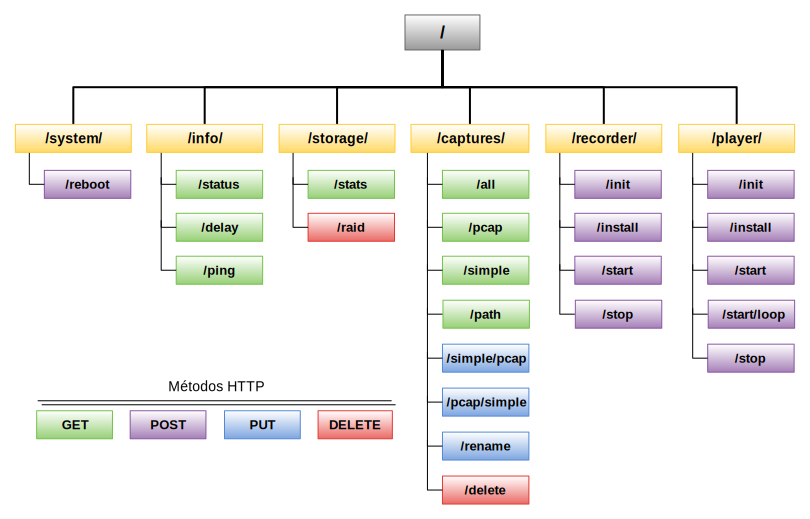
\includegraphics[width=\textwidth,clip=true]{arbol_metodos}
  \caption{Métodos públicos del \gls{servicioweb} \gls{FPGA}.}
  \label{fig:arbol_metodos}
\end{figure}

Arbol rutas \ref{fig:fpga_estado}

\begin{figure}[!htp]
  \centering
  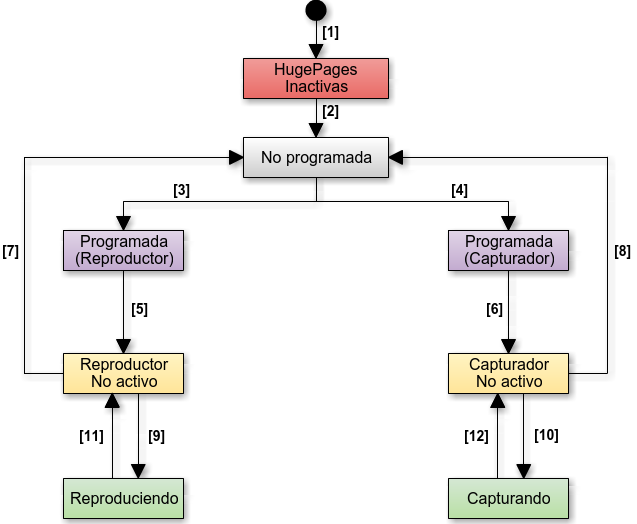
\includegraphics[width=\textwidth,clip=true]{fpga_estado}
  \caption{Máquina de Estados Finita para el estado de la \gls{FPGA}.}
  \label{fig:fpga_estado}
\end{figure}

FSM de estados FPGA \ref{fig:fpga_estado}

Captura árbol de archivos \ref{fig:arbol_codigo}

\begin{figure}[!htp]
  \begin{center}
    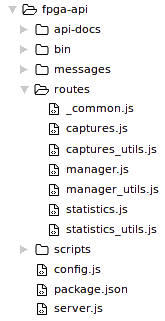
\includegraphics[width=0.3\textwidth,clip=true]{capturas/arbol_backend}
    \hspace{1cm}
    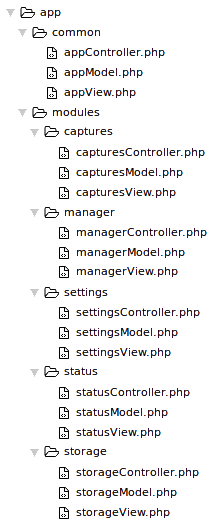
\includegraphics[width=0.3\textwidth,clip=true]{capturas/arbol_frontend}
  \caption{Árboles con los principales archivos de código del \gls{back-end} (a la izquierda) y del \gls{front-end} (a la derecha).}
  \label{fig:arbol_codigo}
  \end{center}
\end{figure}


\section{Front-End\label{sec:imp:front_end}}

Introducción

Resultado Capturas diseño responsive (misma página desde dos sitios) \ref{fig:captura:movil}
\begin{figure}[!htp]
  \centering
  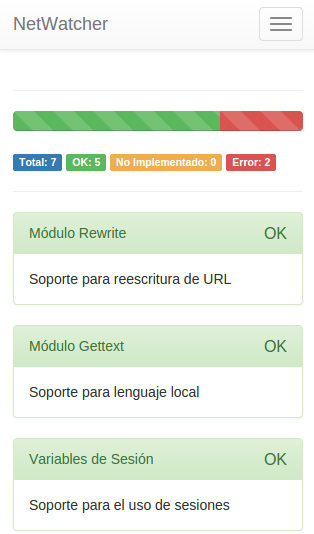
\includegraphics[width=0.4\textwidth,clip=true]{capturas/estado_movil}
  \caption{Página de la aplicación visualizada desde un dispositivo móvil.}
  \label{fig:captura:movil}
\end{figure}

Stack de librerías: MVC propio,Bootstrap,jQuery,gettext, etc.

Captura árbol de archivos \ref{fig:arbol_codigo}

Internacionalización

Temas (captura algún temas) \ref{fig:captura:oscuro}
\begin{figure}[!htp]
  \centering
  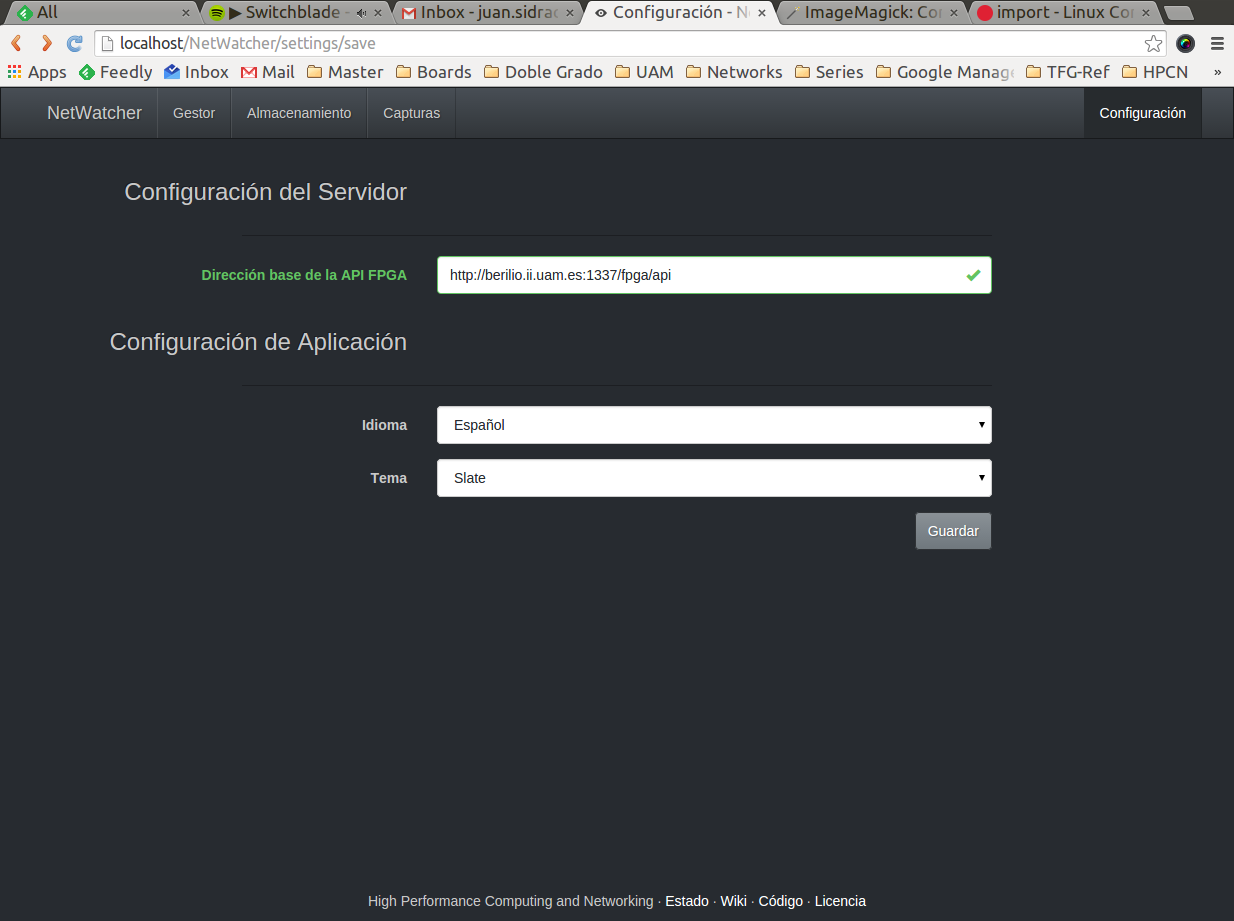
\includegraphics[width=0.95\textwidth,clip=true]{capturas/configuracion_tema_oscuro}
  \caption{Página de la aplicación con un tema oscuro seleccionado.}
  \label{fig:captura:oscuro}
\end{figure}


\section{Documentación \label{sec:imp:docs}}

Se ha creado distinta documentación del proyecto según a quién esté dirigida.
Por un lado, se ha escrito un manual de usuario (disponible en el apéndice \ref{extra:manual_de_usuario}), que pretende ser una guía completa y suficiente para la instalación, configuración y uso de la aplicación.
Adicionalmente, se han publicado en el repositorio de \textit{GitHub} del proyecto (\url{github.com/JSidrach/NetWatcher}) una serie de páginas en formato \textit{wiki} (ver Figura \ref{fig:captura:wiki}). Estas páginas, en inglés, recogen los aspectos más importantes de la aplicación, tanto para el usuario final como para desarrolladores.

\begin{figure}[!htp]
  \centering
  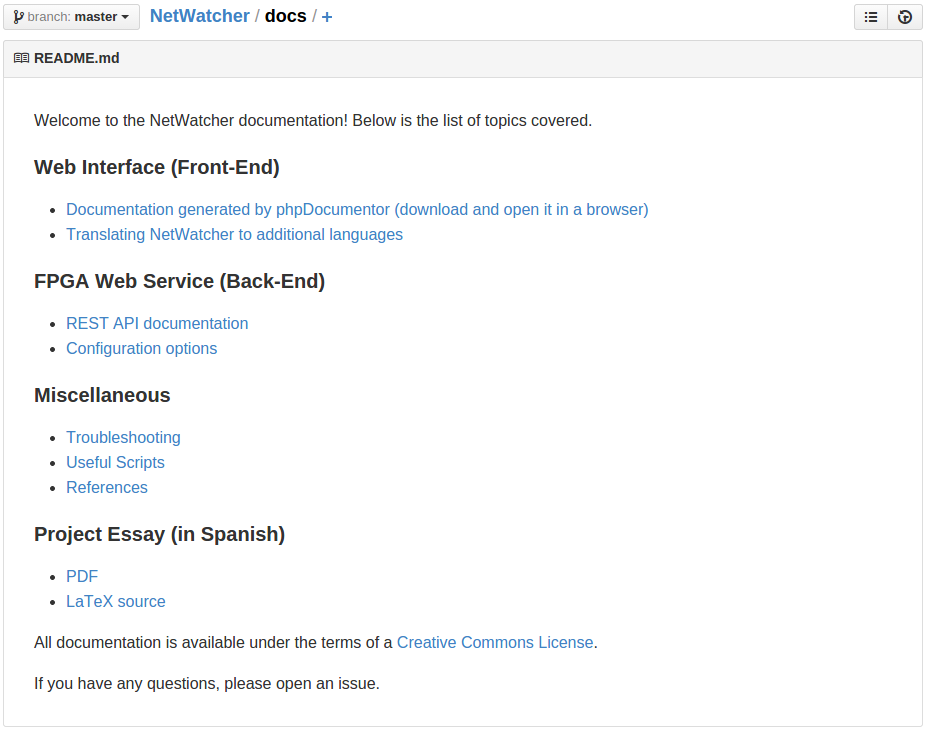
\includegraphics[width=0.95\textwidth,clip=true]{graphics/capturas/github_docs}
  \caption{Captura de una de las páginas de la wiki del proyecto.}
  \label{fig:captura:wiki}
\end{figure} 

A nivel específico de desarrollador, se han utilizado dos herramientas para crear la documentación interna, accesible a través del navegador y en inglés. 
La documentación del \gls{front-end} se ha generado con \textit{phpDocumentor} (ver Figura \ref{fig:captura:docsfrontend}), y la del \gls{back-end} con \textit{apiDoc}.
Esta última se adjunta también, traducida al español, en el apéndice \ref{extra:api_servicio_web_fpga}.
Por último, en el apéndice \ref{extra:frameworkDesarrollado} se explican la arquitectura y funcionalidad del \gls{framework} base para el \gls{front-end}.

\begin{figure}[!htp]
  \centering
  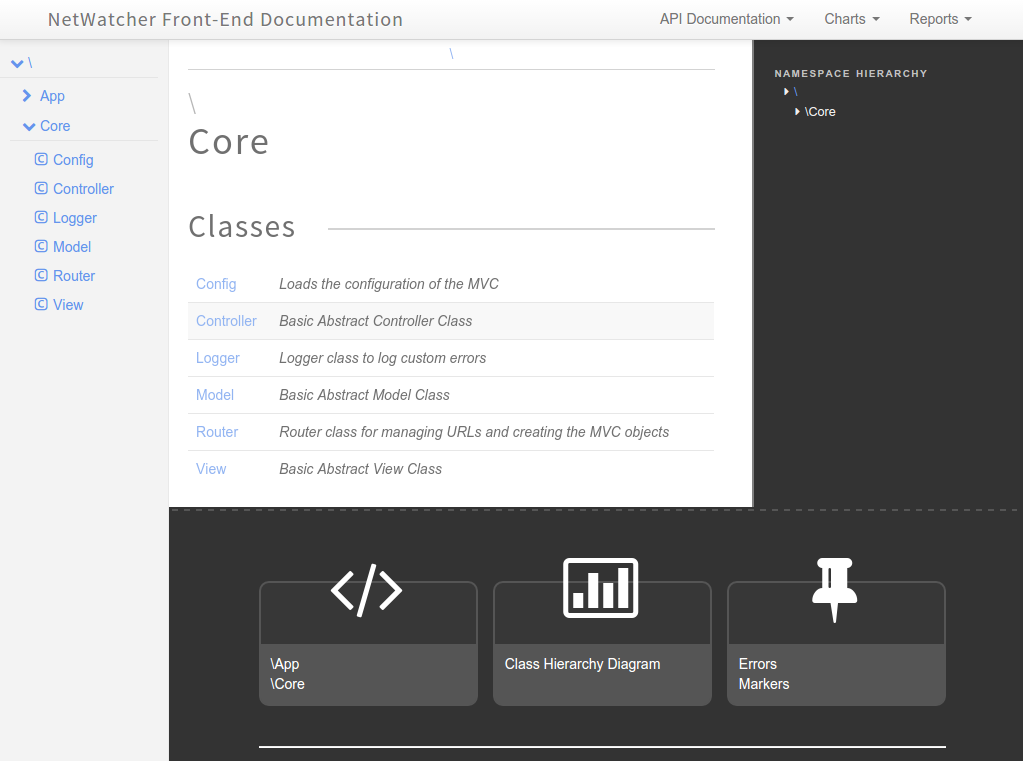
\includegraphics[width=0.95\textwidth,clip=true]{graphics/capturas/docs_frontend}
  \caption{Documentación web del \gls{front-end}.}
  \label{fig:captura:docsfrontend}
\end{figure} 

\chapter{Pruebas\label{cap:pruebas}}

TODO: [Introducción]


\section{Pruebas de verificación\label{sec:pb:verificacion}}

TODO: Pruebas de verificación


\section{Pruebas de validación\label{sec:pb:validacion}}

TODO: Pruebas de validación
\chapter{Mantenimiento\label{cap:mantenimiento}}

TODO: [Introducción]
  {Open Source/GitHub Issues/Pull Requests}
\chapter{Uso de la aplicación\label{cap:uso_de_la_aplicacion}}

TODO: [Introducción]


\section{Instalación\label{sec:uso:instalacion}}

TODO: Instalación


\section{Configuración\label{sec:uso:configuracion}}

TODO: Configuración


\section{Casos de uso\label{sec:uso:casos_de_uso}}

TODO: Casos de uso
  {Apéndice Manual de Usuario}
\chapter{Conclusiones\label{cap:conclusiones}}

TODO: Conclusiones sobre el trabajo realizado
\chapter{Líneas de trabajo futuras\label{cap:lineas_de_trabajo_futuras}}

En el contexto de este Trabajo de Fin de Grado, se ha desarrollado una interfaz web para el manejo de sondas red de altas prestaciones. Sin embargo, el tiempo disponible para ello ha sido limitado, surgiendo diversos ámbitos susceptibles a mejora y ampliación. Por ello, se han identificado áreas de interés que podrían ser consideradas con el objetivo de mejorar la aplicación en el futuro.


\subsection*{Estandarización del Servicio Web}

La aplicación implementada gestiona un dispositivo concreto de captura y reproducción de tráfico de red. Aunque algunos componentes son específicos para la \gls{FPGA} utilizada, también se han desarrollado componentes más genéricos como los de gestión de capturas o almacenamiento. Es por ello que una posible área de mejora es estandarizar el \gls{servicioweb}, documentando los métodos mínimos necesarios para el funcionamiento del servicio de forma genérica. Esto facilitaría la tarea de añadir una interfaz gráfica a otros dispositivos de reproducción y captura de tráfico de red.


\subsection*{Soporte de subtipos de trazas pcap adicionales}

El sistema de gestión de \glspl{traza} actual soporta los formatos \gls{simple} y \gls{pcap}. Las \glspl{traza} en formato \gls{pcap} tienen sin embargo subtipos, cada uno con características distintas que en el sistema actual se descartan. En línea con la estandarización del \gls{servicioweb}, poder distinguir entre los distintos subtipos de \glspl{traza} \gls{pcap} facilitaría obtener información adicional propia de cada subformato, permitiendo además clasificar y convertir entre cada uno de los subtipos.


\subsection*{Registro de estadísticas adicionales}

El sistema actual consta de un módulo que proporciona estadísticas en tiempo real sobre el estado de la \gls{FPGA} y de los distintos componentes que intervienen en el proceso de captura y reproducción. Estos datos no se almacenan de forma persistente una vez obtenidos. Una opción sería guardar en una base de datos estas estadísticas y parámetros de utilización de la \gls{FPGA}. Esto permitiría un análisis posterior de estas estadísticas almacenadas para sacar conclusiones sobre distintos parámetros como el rendimiento o las operaciones más frecuentes.


\subsection*{Localización en otros idiomas}

El trabajo base para dar soporte a diferentes idiomas en la interfaz gráfica ya ha sido realizado, y actualmente la aplicación está disponible en español e inglés. Por tanto, es posible añadir idiomas adicionales a la interfaz traduciendo las distintas cadenas de texto a otros idiomas, sin ser necesario esfuerzo adicional a nivel de diseño e implementación.


\subsection*{Módulo de autenticación}


Dado que la interfaz web está pensada para ser utilizada en redes internas, sin acceso desde exterior, no se ha planteado implementar un módulo de autenticación que impida a usuarios no autorizados el acceso a la aplicación. Desarrollar este módulo de autenticación haría posible instalar el servidor en una dirección pública, sin ceder por ello el control del sistema a una persona ajena. Esto permitiría que un usuario autorizado pudiera utilizar la interfaz desde cualquier punto con conexión a internet.

%
% Página en blanco
%
\cleardoublepage

%
% Bibliografía
%
\bibliography{src/bibliografia}
\addcontentsline{toc}{chapter}{Bibliografía}

%
% Apéndices
%
\appendix
\cleardoublepage
\addappheadtotoc
\appendixpage

%
% Apéndices del TFG
%
\chapter{Ejemplos de bloques y comandos útiles en LaTeX\label{extra:ejemplos}}
\section{Ejemplo de sección}

%
% Breve guía de comandos útiles para la memoria
%

% Citar una referencia
La DARPA creo el protocolo de Internet \cite{ipv4sta}.

% Citar un elemento del glosario
Citamos el acrónimo \gls{FPGA}.

% Citar un elemento del glosario (primera letra en may´usculas)
\Gls{bitstream} es una secuencia de bits.

% Insertar una imagen con pie de página
\begin{figure}[htp!]
  \centering
  
\includegraphics[width=0.75\textwidth,clip=true]{Logo_UAM}
  \caption{Logo de la Universidad Autónoma de madrid.}
  \label{fig:logo_uam}
\end{figure} 

% Referenciar una etiqueta (label)
La figura~\ref{fig:logo_uam} se utiliza en la portada.

% Nueva página
\clearpage

% Añadir código fuente sin líneas
\begin{lstlisting}[label=algoritmo:quicksort,language=C,frame=single,caption=Algoritmo de ordenación Quicksort]
#include <stdio.h>
 
void quick_sort (int *a, int n) {
    int i, j, p, t;
    if (n < 2)
        return;
    p = a[n / 2];
    for (i = 0, j = n - 1;; i++, j--) {
        while (a[i] < p)
            i++;
        while (p < a[j])
            j--;
        if (i >= j)
            break;
        t = a[i];
        a[i] = a[j];
        a[j] = t;
    }
    quick_sort(a, i);
    quick_sort(a + i, n - i);
}
\end{lstlisting}

% Fórmula dentro de una línea de texto
La ecuación de Euler ($e^{ \pm i\theta } = \cos \theta \pm i\sin \theta$) es citada frecuentemente como un ejemplo de belleza matemática.

% Fórmula independiente
\begin{equation}\label{eq:pythagoras}
a^2 + b^2 = c^2
\end{equation} % TODO: borrar
\chapter{Manual de Usuario\label{extra:manual_de_usuario}}

TODO: [Introducción]
  {Descripción detallada}
\chapter{Framework MVC propio\label{extra:framework_mvc_propio}}

TODO: [Introducción]
  {Visión global}


\section{Modelo Vista Controlador\label{extra:sec:mvc}}

TODO: Modelo Vista Controlador


\section{Manejo de dependencias\label{extra:sec:dependencias}}

TODO: Manejo de dependencias


\section{Config\label{extra:sec:config}}

TODO: Config


\section{Router\label{extra:sec:router}}

TODO: Router


\section{Logger\label{extra:sec:logger}}

TODO: Logger


\section{Conclusiones\label{extra:sec:conclusiones}}

TODO: Conclusiones
\chapter{Programación asíncrona\label{extra:programacion_asincrona}}

TODO: Programación asíncrona
\chapter{API Servicio Web FPGA\label{extra:api_servicio_web_fpga}}

TODO: API Servicio Web FPGA

{captures,manager,statistics}

% Fin del documento
\end{document}